\documentclass[11pt]{article}

\usepackage{amsmath,amssymb}
\usepackage[margin=0.85in]{geometry}
\usepackage{tikz}
\usetikzlibrary{arrows.meta, positioning, calc}
\usepackage{enumitem}

\pagestyle{empty}

\title{Algorithm: Multilayer to Homogeneous Voigt Rheology}
\author{}
\date{}

\begin{document}
\maketitle
\thispagestyle{empty}

%======================================================================
% Page 1: Schematic overview
%======================================================================

\vspace{-1.5em}
\begin{center}
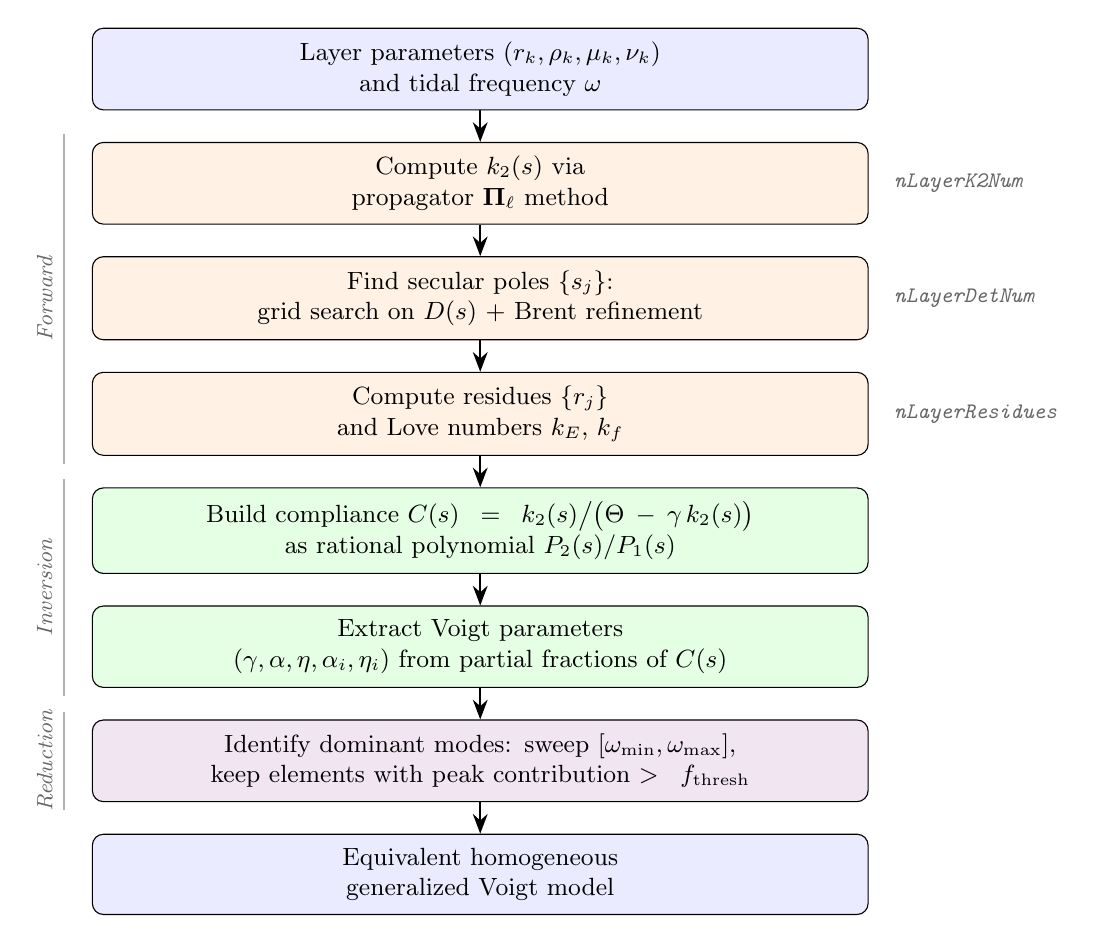
\begin{tikzpicture}[
  box/.style={draw, rounded corners, text width=9.5cm,
              minimum height=0.9cm, align=center, font=\small,
              inner sep=5pt},
  arrow/.style={-{Stealth[length=2.5mm]}, thick},
  lbl/.style={font=\footnotesize\itshape, text=black!60},
  node distance=0.4cm
]

\node[box, fill=blue!8] (input)
  {Layer parameters $(r_k, \rho_k, \mu_k, \nu_k)$\\
   and tidal frequency $\omega$};

\node[box, fill=orange!10, below=of input] (k2)
  {Compute $k_2(s)$ via\\propagator $\mathbf{\Pi}_\ell$ method};
\node[lbl, right=0.2cm of k2] {\texttt{nLayerK2Num}};

\node[box, fill=orange!10, below=of k2] (poles)
  {Find secular poles $\{s_j\}$:\\grid search on $D(s)$ $+$ Brent refinement};
\node[lbl, right=0.2cm of poles] {\texttt{nLayerDetNum}};

\node[box, fill=orange!10, below=of poles] (res)
  {Compute residues $\{r_j\}$\\and Love numbers $k_E$, $k_f$};
\node[lbl, right=0.2cm of res] {\texttt{nLayerResidues}};

\node[box, fill=green!10, below=of res] (C)
  {Build compliance $C(s) = k_2(s)\big/\bigl(\Theta - \gamma\, k_2(s)\bigr)$\\
   as rational polynomial $P_2(s)/P_1(s)$};

\node[box, fill=green!10, below=of C] (voigt)
  {Extract Voigt parameters\\
   $(\gamma, \alpha, \eta, \alpha_i, \eta_i)$
   from partial fractions of $C(s)$};

\node[box, fill=violet!10, below=of voigt] (dom)
  {Identify dominant modes: sweep $[\omega_{\min}, \omega_{\max}]$,\\
   keep elements with peak contribution $> f_{\mathrm{thresh}}$};

\node[box, fill=blue!8, below=of dom] (output)
  {Equivalent homogeneous\\generalized Voigt model};

\draw[arrow] (input) -- (k2);
\draw[arrow] (k2) -- (poles);
\draw[arrow] (poles) -- (res);
\draw[arrow] (res) -- (C);
\draw[arrow] (C) -- (voigt);
\draw[arrow] (voigt) -- (dom);
\draw[arrow] (dom) -- (output);

% Left-side stage lines and centered labels
\coordinate (fwdTop) at ($(k2.north west)+(-0.35,0.1)$);
\coordinate (fwdBot) at ($(res.south west)+(-0.35,-0.1)$);
\draw[thick, black!30] (fwdTop) -- (fwdBot);
\node[lbl, rotate=90] at ($(fwdTop)!0.5!(fwdBot)+(-0.25,0)$) {Forward};

\coordinate (invTop) at ($(C.north west)+(-0.35,0.1)$);
\coordinate (invBot) at ($(voigt.south west)+(-0.35,-0.1)$);
\draw[thick, black!30] (invTop) -- (invBot);
\node[lbl, rotate=90] at ($(invTop)!0.5!(invBot)+(-0.25,0)$) {Inversion};

\coordinate (redTop) at ($(dom.north west)+(-0.35,0.1)$);
\coordinate (redBot) at ($(dom.south west)+(-0.35,-0.1)$);
\draw[thick, black!30] (redTop) -- (redBot);
\node[lbl, rotate=90] at ($(redTop)!0.5!(redBot)+(-0.25,0)$) {Reduction};

\end{tikzpicture}
\end{center}

\vspace{0.5em}
\noindent{\small\textbf{References.}\;
\textit{Gevorgyan, Matsuyama \& Ragazzo (2023), MNRAS 523, 1822.}\\
\textit{Sabadini, Vermeersen \& Cambiotti (2016), Global Dynamics of
the Earth, 2nd ed., Springer.}}

\newpage

%======================================================================
% Page 2: Full algorithm
%======================================================================

\section*{Full algorithm}

\subsection*{Notation}

Layered-body quantities follow Sabadini, Vermeersen \& Cambiotti
(2016): $\mu_k$~shear modulus, $\nu_k$~viscosity,
$\mathbf{Y}_\ell$~fundamental matrix,
$\mathbf{\Pi}_\ell$~propagator, $\mathbf{I}_C$~core boundary matrix,
$D(s)$~secular determinant.  Homogeneous-body quantities follow
Gevorgyan, Matsuyama \& Ragazzo (2023, hereafter GMR\,2023):
$C(s)$~compliance, $P_1(s)$/$P_2(s)$~polynomials, $\gamma$, $\alpha$,
$\eta$, $\alpha_i$, $\eta_i$~Voigt parameters.

\subsection*{Input}
Layer parameters $\{r_k, \rho_k, \mu_k, \nu_k\}_{k=1}^{N}$
(center to surface), tidal frequency $\omega$, working precision
$p$, pole-search grid bounds $[a_{\min}, a_{\max}]$ with $G$ points,
frequency interest range $[\omega_{\min}, \omega_{\max}]$, dominant
threshold $f_{\mathrm{thresh}}$.

\subsection*{Stage 1: Forward problem}

\begin{enumerate}[leftmargin=2em]
  \item For each layer $k$, form the Maxwell complex shear modulus
    via the Correspondence Principle:
    $\hat\mu_k(s) = \mu_k \nu_k s / (\mu_k + \nu_k s)$.
    For liquid layers ($\mu_k < 1$\,Pa), regularize
    $\hat\mu_k \approx 10^{-20}$\,Pa.

  \item Build the $6\times6$ fundamental matrix
    $\mathbf{Y}_\ell(r)$ for each layer
    (degree $\ell = 2$; Sabadini et al.\ 2016, Eq.~2.42),
    where each column is an independent solution of the
    spheroidal system within that layer.

  \item Form the propagator
    $\mathbf{\Pi}_\ell(r, r') =
    \mathbf{Y}_\ell(r)\,\mathbf{Y}_\ell^{-1}(r')$ (Eq.~2.9)
    and chain through all $N$ layers from the core--mantle boundary
    matrix $\mathbf{I}_C$ (Eq.~2.6) to the surface.

  \item Compute the secular determinant
    $D(s) = \det\bigl(\mathbf{P}_1\,\mathbf{\Pi}_\ell(R, r_C)\,
    \mathbf{I}_C\bigr)\big|_{\mu=\hat\mu(s)}$ (Eq.~1.199) and
    extract $k_2(s)$ from the surface boundary conditions.
\end{enumerate}

\subsection*{Stage 2: Modal decomposition}

\begin{enumerate}[leftmargin=2em, resume]
  \item Evaluate $k_E = \mathrm{Re}[k_2(10^{10})]$ (elastic limit)
    and $k_2(i\omega)$ at the tidal frequency.

  \item Build a logarithmic grid $s_n = -10^{a_n}$ with $G$ points
    in $[a_{\min}, a_{\max}]$.  Evaluate $D(s_n)$ at each grid point.

  \item Detect sign changes in $D(s)$ between
    consecutive grid points.  Refine each bracket with Brent's method
    to obtain all $M$ secular poles $\{s_j\}$, $s_j < 0$
    (Sabadini et al.\ 2016, Eq.~1.200).

  \item For each pole, compute the residue via the limit formula:
    $r_j = \delta \cdot k_2(s_j + \delta)$ with
    $\delta = 10^{-6}|s_j|$.

  \item Compute the fluid Love number
    $k_f = k_E + \sum_{j=1}^{M}(-r_j / s_j)$.
    The partial-fraction form is
    (GMR\,2023, Eq.~26):
    $k_2(s) = k_E + \sum_{j=1}^{M} r_j/(s - s_j)$.
\end{enumerate}

\subsection*{Stage 3: Rheological inversion}

\begin{enumerate}[leftmargin=2em, resume]
  \item Compute mapping constants
    (GMR\,2023, Eqs.~2,\,4):
    $\Theta = 3\mathrm{I}_\circ G/R^5$,\;
    $\gamma = \Theta / k_f$,\;
    $\alpha = \Theta / k_E - \gamma$.

  \item Build the compliance as a rational polynomial
    (GMR\,2023, Eq.~6):
    $C(s) = P_2(s) / P_1(s)
    = k_2(s) / (\Theta - \gamma\, k_2(s))$,
    using the partial-fraction form of $k_2$.

  \item Factor the $s = 0$ root from $P_1(s)$ to
    extract the isolated dashpot parameter $\eta$.

  \item Solve $P_2(s) = 0$ for the $N_V = M-1$
    Voigt poles $\{q_i\}$, $q_i < 0$ (GMR\,2023, Eq.~20).

  \item For each Voigt pole, extract the spring and dashpot
    compliance parameters $\alpha_i$, $\eta_i$ from the
    partial-fraction coefficients of $C_v(s)$ (Eq.~23);
    characteristic time $\omega_i^{-1} = \eta_i / \alpha_i$ (Eq.~18).

  \item Convert from compliance space to physical units:
    multiply $\gamma$, $\alpha$, $\eta$, $\alpha_i$, $\eta_i$ by
    $F = 5\bar\rho R^2 / 38$.
\end{enumerate}

\subsection*{Stage 4: Dominant mode selection}

\begin{enumerate}[leftmargin=2em, resume]
  \item Sweep 200 log-spaced frequencies in
    $[\omega_{\min}, \omega_{\max}]$.

  \item At each frequency, compute each Voigt element's fractional
    contribution to $-\mathrm{Im}[C(i\omega)]$.

  \item Record the maximum fractional contribution of each element
    across the sweep.

  \item Retain element $i$ if
    $\max_\omega\bigl(-\mathrm{Im}[C_i] / -\mathrm{Im}[C]\bigr) >
    f_{\mathrm{thresh}}$.

  \item Build the reduced model from the spring $1/\alpha$, the
    dashpot $1/(\eta\,s)$, and the retained Voigt elements.
\end{enumerate}

\subsection*{Output}

\begin{itemize}[leftmargin=2em]
  \item Love numbers: $k_E$, $k_f$, $k_2(i\omega)$.
  \item Full Voigt model: $\gamma$, $\alpha$, $\eta$,
    $\{(\alpha_i, \eta_i, \omega_i^{-1})\}_{i=1}^{N_V}$.
  \item Secular poles and residues: $\{(s_j, r_j)\}_{j=1}^{M}$.
  \item Reduced Voigt model: dominant elements only, with
    $k_2$ comparison and relative errors.
  \item Comparison plots: $\mathrm{Re}[k_2]$ and
    $-\mathrm{Im}[k_2]$ vs $\omega$ for full and reduced models.
\end{itemize}

\end{document}
